\documentclass[12pt]{report}
\usepackage{graphicx}
\usepackage{titling}
\usepackage{fancyhdr}
\usepackage[latin1]{inputenc}
\usepackage{enumerate}
\usepackage{float}
\usepackage{latexsym}
\usepackage{amssymb}
\usepackage{amsthm}
\usepackage{amsfonts}
\usepackage{amsmath}
\usepackage[usenames,dvipsnames,svgnames,table]{xcolor}
\usepackage{listings}
\parindent=0pt
\frenchspacing

\pagestyle{fancy}

\fancyhead[L]{\slshape\footnotesize December 3, 2013\\\textsc{02246 Model Checking}}
\fancyhead[R]{\slshape\footnotesize \textsc{Andreas Kjeldsen (s092638)}\\\textsc{Morten Eskesen (s133304)}}
\fancyfoot[C]{\thepage}

\lstdefinestyle{prismmodel}{
	tabsize=1,
	captionpos=b
  	belowcaptionskip=1\baselineskip,
  	breaklines=true,
  	frame=single,
	frameround=tttt,
	captionpos=b,
  	language={},
  	numbers=left,
  	numbersep=5pt,
  	numberstyle=\tiny\ttfamily\color{Black},
  	basicstyle=\footnotesize\ttfamily\color{Black},
  	keywordstyle=\bfseries\color{Black},
	morekeywords={module, endmodule, label, init, mdp }, 
	otherkeywords={=, :, [, ], |},
	identifierstyle={\color{red}\let\textcolor\textcolordummy},
	morestring=[b][\color{red}\bfseries]",
	commentstyle=\color{Green},
	moredelim=[s][\color{DarkOrchid}\ttfamily]{[}{]},
	literate=%
		*{0}{{{\color{blue}0}}}1
	    {1}{{{\color{blue}1}}}1
	    {2}{{{\color{blue}2}}}1
	    {3}{{{\color{blue}3}}}1
	    {4}{{{\color{blue}4}}}1
	    {5}{{{\color{blue}5}}}1
	    {6}{{{\color{blue}6}}}1
	    {7}{{{\color{blue}7}}}1
	    {8}{{{\color{blue}8}}}1
	    {9}{{{\color{blue}9}}}1
}

\newcommand{\tab}{\hspace*{2em}}
\newcommand{\HRule}{\rule{\linewidth}{0.5mm}}

\begin{document}

\begin{titlepage}
\begin{center}


\includegraphics[scale=2.0]{../GFX/dtu_logo.pdf}\\[1cm]

\textsc{\LARGE Technical University of Denmark}\\[1.5cm]

\textsc{\Large 02246 Model Checking}\\[0.5cm]


% Title
\HRule \\[0.4cm]
{\huge \bfseries Mandatory Assignment\\Part 2: Stochastic Modelling and Verification in Discrete Time}\\[0.1cm]
\HRule \\[1.5cm]

% Author and supervisor
\large
\emph{Authors:}
\\[10pt]
Andreas Hallberg \textsc{Kjeldsen}\\
\emph{s092638@student.dtu.dk}
\\[10pt]
Morten Chabert \textsc{Eskesen}\\
\emph{s133304@student.dtu.dk}

\vfill

% Bottom of the page
{\large December 3, 2013}

\end{center}
\end{titlepage}

\chapter*{Introductory notes}
This report has been written by the both of us. All parts have been worked on together and therefore our responsibility for each assignment is equal.
\chapter*{Part A: Introductory Problems}
\section*{A1) Practical Problems}

\subsection*{A1.1}
In this problem we will ad probabilities to the FCFS scheduler from the previous assignment, so that we construct a discrete time Markov chain.

\subsubsection*{A1.1a)}
Currently in the FCFS scheduler there are sources of non-determinism. Some of the sources are the create commands in $client_1$ and $client_2$ because there are 5 different create commands with the same guard only the update distinguishes the commands. These sources are due to local non-determinism between the commands in the modules. The other source of non-determinism is due to concurrent execution of the modules in FCFS. The shifting command in the Scheduler module is a result of non-determinism because it can happen independently of what the other modules are doing.

\subsubsection*{A1.1b)}
In order to resolve the local non-determinism we have to modify the modules to include probabilistic commands. Since the distribution of the probabilities should be uniform the new create command will look like the following:
\begin{lstlisting}[style=prismmodel]
[create1] state1=0 -> 0.2 :(state1'=1) & (task1'=1) +
                      0.2 :(state1'=1) & (task1'=2) +
                      0.2 :(state1'=1) & (task1'=3) +
                      0.2 :(state1'=1) & (task1'=4) + 
                      0.2 :(state1'=1) & (task1'=5);
\end{lstlisting}

\subsubsection*{A1.1c)}
The FCFS file has been changed to have the extension .pm and the first line of the model is 'dtmc' which tells PRISM that the file describes a Discrete Time Markov Chain. Building the model causes no errors and tells us that we now have 83 reachable states in the model. Which was the same as before because PRISM resolves the local non-determinism by using a uniform distribution. If there are 5 possibilities it will choose each with probability $\frac{1}{5}$.

\subsubsection*{A1.1d)}
As explained earlier the shifting command in the Scheduler module causes some non-determinism. This non-determinism we have due to the concurrent execution of the modules is still there. If there were commands in the other commands in the modules that could happen independently of what the Scheduler module was doing all of these commands would happen with equal probability. Since there are no other commands specified that way the command in the Scheduler module happens with probability 1 when possible. PRISM enforces this.

\subsubsection*{A1.1e)}
In order to make sure that a job will almost certainly complete we specify the following PRISM properties - one for each client.
\begin{center}
$(task_1 > 0) \Rightarrow P_{\geq 1}(F(task_1 = 0))$\\
$(task_2 > 0) \Rightarrow P_{\geq 1}(F(task_2 = 0))$
\end{center}
These properties have been verified by PRISM so we now know that a created job will almost certainly complete in this model.

\subsection*{A1.2}
This section is about using PRISM to compute numerical properties of the FCFS model.

\subsubsection*{A1.2a)}
If we calculate the steady state distribution of the model we can find the probability of having no jobs in the scheduler. We use PRISM to calculate the steady state distribution and it gives us the probability of being in each of the reachable states. Only one state has no jobs in the scheduler which is the initial:
\begin{center}
0:(0,0,0,0,0,0)=0.016145825133811565
\end{center}
The probability of having no jobs in the scheduler is therefore 0.0161.

\subsubsection*{A1.2b)}
We want to calculate the expected length of a job for $client_1$ by looking at the steady state probabilities. In order to do this computation manually we first have to sum the probabilities of the states where $client_1$ has a job of length $i$, $0 \leq i \leq 5$. These states are states 12-82.
\begin{center}
Probability: 0.75
\end{center}

$$\frac{0 * 0.0911 + 1 * 0.1675 + 2 * 0.1506\\+ 3 * 0.1331 + 4 * 0.1142 + 5 * 0.0935}{0.75} = 2.39$$
The expected length of a job for $client_1$ is 2.39.

\subsubsection*{A1.2c)}
We want to know what the probability of $client_1$ not having a job at time $t = 10$ so we calculate the transient distribution of the model at time $t = 10$. When we do this PRISM will output the probability for being in each state at this time and we sum the probabilities of being in states where $client_1$ does not have a job. States where $client_1$ does not have a job are states 0-11. We sum the probability of being in these states and get:
\begin{center}
Probability: 0.2574
\end{center}

\subsubsection*{A1.2d)}
We have to plot a graph of the probability that $client_1$ does not have a job against time $t$, for $0 \leq t \leq 10$. We therefore calculate the transient distribution of the model for time $t$. We sum the probabilities of the states where $client_1$ does not have a job. We can then plot the graph of the probability.\\
\begin{figure}[H]
	\centering
	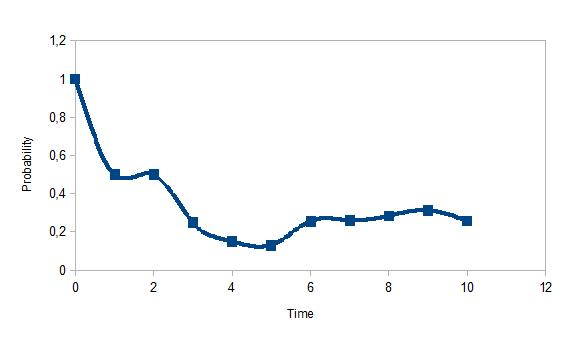
\includegraphics[scale=0.9]{../GFX/A1-2d.png}\\
	Figure A1.2d: The graph
\end{figure}
The graph starts a probability 1 because in the initial state there is no jobs in the scheduler. Then the probability falls to 0.5 because there is an equal probability of $client_1$ and $client_2$ creating a job. After that the probability is between 0.15 and 0.30 which is quite low because each client can always have one job in the scheduler therefore there is a higher probability of the clients having a job in the scheduler.

\subsection*{A1.3}
This part is about PCTL model checking in PRISM. We will specify some PCTL formula about the FCFS. For each PCTL formula we will explain what the PCTL formula captures. We will use PRISM to determine whether the \emph{initial state} of the model satisfies it.

\begin{description}
\item[A1.3a)] $$P > 0.2 (\bigcirc task1 > 2)$$
This PCTL formula captures a query that asks if the probability is greater than 0.2 that $client_1$ will have an active job of length greater than 2 in the next time unit. This has been verified by PRISM for the model.


\item[A1.3b)] $$P < 0.5 (\Diamond^{\leq10} task2=5)$$
This PCTL formula captures a query that asks if the probability is less than 0.5 that $client_2$ will create a job of length 5 within 10 time units. This has been verified by PRISM for the model.


\item[A1.3c)] $$P > 0 (\Box state1=1)$$
This PCTL formula captures a query that asks if the probabilty is greater than zero that $client_1$ will always have an active job. This has not been verified by PRISM as it is false.


\item[A1.3d)] For all of the above properties we use the '$P=?$' notation in PRISM to calculate the actual probability.
\begin{center}
\begin{tabular}{l c}
PCTL formula & Probability\\
$P=?(\bigcirc task1> 2)$ & 0.3\\
$P=?(\Diamond^{\leq10} task2=5)$ & 0.26\\
$P=?(\Box state1=1)$ & 0.0\\
\end{tabular}
\end{center}

\end{description}

\subsection*{A1.4}
In the first part of the course we used the syntax '$P>=1$' and '$!P<=0$' to encode the quantifiers $A$ and $E$ when we wrote CTL formulae in PRISM. If we want to model check CTL formulae on a DTMC, however, these do not encode the $A$ and $E$ quantifiers as we would expect.

\subsubsection*{A1.4a)}
A DTMC satisfies a CTL formula if the transition system obtained by throwing away the probabilities in the DTMC satisfies the formula. Formally this can be written as:
$$Sat_{TS(M)}(\Psi),$$
where TS(M) is the transition system obtained by throwing away the probabilities in Markov Chain $M$ and $\Psi$ is the CTL formula.

\subsubsection*{A1.4b)}
Considering the CTL formula $EG s_0$ and the PCTL formula $\neg P_{\leq 0}(G s_0)$. In the figure below a DTMC is described where the CTL formula holds but the PCTL formula does not hold.
%%%%FIGUR

\subsubsection*{A1.4c)}
The CTL formula holds because there exists a path from $s_0$ where for the rest of time $s_0$ will be satisfied which is because it will loop forever. Where as the PCTL formula has probability and it is therefore unlikely that it will loop forever.

\subsubsection*{A1.4d)}
The quantifier $E$ is required in order for the semantics of these formulae to be the same. Because since there are probabilities involved there will aways be a chance that it will step out of the loop. Meanwhile in CTL there should just be a path that satisfies the specified property.

\section*{A2) Theoretical Problems}
\subsection*{A2.1}

\subsubsection*{A2.1a)}


\subsubsection*{A2.1b)}


\subsubsection*{A2.1c)}

\subsection*{A2.2}


\subsection*{2A.3}

\subsubsection*{2A.3a)}

\subsubsection*{2A.3b)}


\subsubsection*{2A.3c)}


\subsection*{2A.4}

\subsubsection*{2A.4a)}

\subsubsection*{2A.4b)}

\chapter*{Part B: Intermediate Problems}
\section*{B1) Practical Problems}
\subsection*{Lottery scheduler}
In this part we will model a Lottery Scheduler (found in the LotteryScheduler.pm file). In Lottery Scheduling each task is assigned a number of tickets. When the scheduler has to decide which task to execute, the scheduler selects a ticket under a uniform distribution, and the task owning the ticket is allowed to execute. Our Lottery Scheduler is \emph{pre-emptive} which means that a task can only execute for a certain amount of time before being interrupted. In our scheduler the amount of time is one time unit.  Our Lottery Scheduler has three clients with one task each. Each task has a single ticket. We have modeled the tickets as a single variable in the scheduler module. The variable called \emph{ticket} has a range of 0 to 3 and it is initialized as 0. The serving of the jobs is as follows: Whenever a task is in the scheduler it is allowed to execute for one time unit given that the ticket has a value equal to the client's number. After the job has executed for one time unit the variable ticket is assigned to 0. The exciting part is assigning the value of the ticket.

\begin{lstlisting}[style=prismmodel]
  [] ticket=0 -> 0.333333333333333333333333:(ticket'=1) + 0.333333333333333333333333:(ticket'=2) + 0.333333333333333333333333:(ticket'=3);
  [] job1=false & ticket=1 -> 0.5:(ticket'=2) + 0.5:(ticket'=3);
  [] job2=false & ticket=2 -> 0.5:(ticket'=1) + 0.5:(ticket'=3);
  [] job3=false & ticket=3 -> 0.5:(ticket'=1) + 0.5:(ticket'=2);
\end{lstlisting}
Whenever the ticket is 0 there should be an equal probability of choosing one of the three jobs. But however it is possible that not all clients have a job in the scheduler which is why it is necessary with the other three commands. Here the value of the ticket is assigned with equal probability 0.5 since there are only two jobs in the scheduler.\\

\subsubsection*{Executing time for $client_1$}
We are interested in the time taken for the first task from $client_1$ to complete. In order to do this we introduce a new module called \emph{Monitor}. Monitor has only one variable called finished which is a boolean value. It is initialized as false. When the finish1 command is executed meaning the first job from $client_1$ has completed the finished variable will be set to true. For subsequent actions it remains in this state.\\
We write a PCTL formula using the '$P=?$' syntax expressing that the first task from $client_1$ completes within in $t$ time units. $t$ is defined as an integer constant without a value. We will use the experimentation feature of PRISM to plot a graph of this probability for $0 \leq t \leq 20$.\\
The PCTL formula: $P=? (\Diamond^{\leq t} finished=true)$\\
\begin{figure}[H]
	\centering
	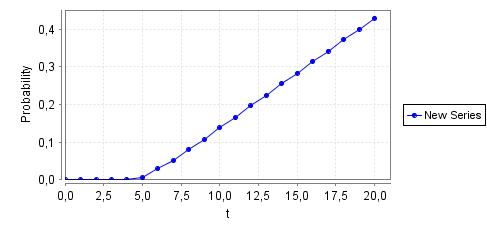
\includegraphics[scale=0.75]{../GFX/B1-1c.png}\\
	Figure B1.1: The graph plotting the probability for $0 \leq t \leq 20$ with one time unit
\end{figure}

\subsubsection*{Starvation}
We are interested in finding out whether it is possible for our lottery scheduler to suffer from starvation. In order to determine this we specify some PCTL formula which we will use PRISM to verify. The PCTL formulae states that whenever task1, task2 or task3 is greater than zero there must be a probability of greater than or equal to 1 that task1, task2 or task3 will eventually be zero. This means that whenever a job is created it will be served until it is finished.
\begin{center}
$(task1 > 0) \Rightarrow P_{\geq 1}(F(task1 = 0))$\\
$(task2 > 0) \Rightarrow P_{\geq 1}(F(task2 = 0))$\\
$(task3 > 0) \Rightarrow P_{\geq 1} (F(task3 = 0))$
\end{center}
These properties have been verified by PRISM so it is not possible in our model that our lottery scheduler will suffer from starvation.

\subsubsection*{Two time units modification}
We wish to modify our allowed time for execution for each task so that is two time units (found in the file LS-2units.pm). We do this by defining an integer variable called \emph{time} with a range between 0 and 2. Whenever the variable ticket is 0 then it will assign ticket to a value according to each client with an equal probability as before but now it will also set the variable time to 2. The guards for the serve commands now have an additional condition which is that time must be greater than 0. Meanwhile whenever time is 0 and ticket is above 0 ticket will be reset to 0 so a new job can be served. Furthermore whenever finish for a job is activated it will reset time to 0. The interesting part is how this affects the time taken to complete a task from $client_1$. We will do the same as before and make a graph.\\
\begin{figure}[H]
	\centering
	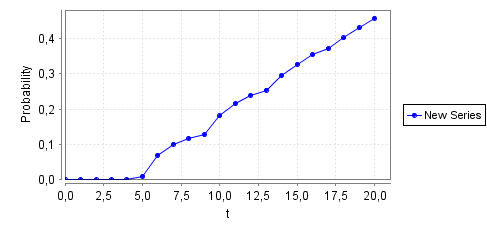
\includegraphics[scale=0.75]{../GFX/B1-1e.png}\\
	Figure B1.2: The graph plotting the probability for $0 \leq t \leq 20$ with two time units
\end{figure}
As we can see by the graph it does not affect the total probability much but the graph has larger spikes in probability because the time unit is now increased by 1.

\subsection*{Priority Lottery Scheduler}
Instead of assigning the same number of tickets to each task we now give varying priority to different tasks by assigning them different numbers of tickets. This variant of the lottery scheduler can be found in the file PLS.pm. We will approximate a Shortest Remaining Time scheduler by using this kind of lottery scheduling. This means that small tasks will be assigned more tickets than a large task. We have done this approximation by creating three integer variables with range from 0 to 5 and they are initialized as 5. These three variables are called ticket1, ticket2 and ticket3 - one for each client. When a client creates a job the client must not have a job in the scheduler already or the client's corresponding ticket may not be any other value than 5. This is because the ticket belonging to the client will get its value by subtracting the length of its job from the ticket's value. Meaning that a job of length 5 will be assigned a ticket value of 0. When the jobs in the scheduler are finished their ticket values will be reset to 5. The serving of the jobs have a guard that specifies that its ticket value must be greater or equal to the other tickets in order to be served.

\subsubsection*{Time taken and Starvation}
We wish to find out how this affects the time taken to complete a task from $client_1$. We will once again plot a graph for the probability.
\begin{figure}[H]
	\centering
	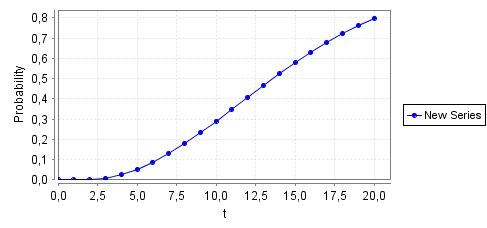
\includegraphics[scale=0.75]{../GFX/B1-2b.png}\\
	Figure B1.3: The graph plotting the probability for $0 \leq t \leq 20$ with priorities
\end{figure}
As we can see by the graph adding priorities will affect the time taken to complete a task from $client_1$. It now has a higher probability of finishing a job within 20 time steps because all the small jobs will be served first by the scheduler.
\\Also we would like to find out if starvation is possible in our model. We therefore use the following PCTL formula to verify the properties in PRISM.
\begin{center}
$(task1 > 0) \Rightarrow P_{\geq 1}(F(task1 = 0))$\\
$(task2 > 0) \Rightarrow P_{\geq 1}(F(task2 = 0))$\\
$(task3 > 0) \Rightarrow P_{\geq 1} (F(task3 = 0))$
\end{center}
These properties have been verified by PRISM meaning that a job will always complete but it is worth noting that it can take a job of length 5 a long time to complete if the other clients keep creating shorter jobs.

\subsubsection*{Investigation of the model}
We want to increase the number of clients in our model until we reach the maximum for which PRISM can still build and solve the underlying DTMC. We do this by just incrementing and building till PRISM cannot build anymore. This gives us a maximum of 8 clients. It takes a time to build the model. With trying to build with 9 clients PRISM shut down with no errors.\\
In general having a scheduler that uses priority based scheduling or a shortest time based scheduling will make the scheduler vulnerable to denial of service attack. Because in our model  if a client tries to perform long jobs but all the other clients generate very short jobs. The short jobs will move ahead of the queue and the long jobs will never be served if there always will be generated more short jobs. It would be desirable to express denial of service as a PCTL property but this is not possible for our model. This is because in our model the job will always complete it is just a question of time. We cannot express a PCTL property that will create a job every time the old short job finished.

\section*{B2) Theoretical Problems}

\subsection*{Bisimulation relations}
We have to consider the DTMC in the figure above, where $s_0$ is the initial state, and the labels are shown on the states. We will call this $M = (S, P, s_0, AP, L)$, where $AP = \{a, b\}$.\\
We write down the coarsest probabilistic bisimuliation relation between the states of $M: R \subseteq S \times S$.
$$R = \{ (s_0, s_0), (s_0,s_5), (s_1,s_1), (s_1,s_4),(s_2,s_2),(s_2,s_3),(s_3,s_3)$$ $$(s_3,s_2),(s_4,s_4),(s_4,s_1),(s_5,s_5),(s_5,s_0)\}$$

This relation is a probabilistic bismulation. This can be seen as follows. States $s_0$ and $s_5$ can move to a state with label $a$ with probability 1. States $s_1$ and $s_4$ can both move to a state with label $b$ with probability 0.8 and to a state with label $a$ with probabilty 0.2. States $s_2$ and $s_3$ can move to a state with label $b$ with probability 0.7 and to a state with label $a$ with probability 0.3.\\
We have constructed the bisimulation quotient $M / \sim$ of $M$. This can be seen in the figure below.\\
%%Indsæt figur tegnet af Andreas her

\chapter*{Part C: Advanced Problems}
\section*{Practical Problems}
In this part we wish to extend our Priority Lottery Scheduler from part B1, where there are multiple servers. This means that we have to seperate the functionality of the scheduler from the execution of the tasks which previously have been combined in the module Scheduler. The scheduler has to decide the order of which the tasks execute and which server executes them. We will modify our lottery scheduler to model a system with two servers. In the following subsections we will describe how the scheduler chooses the order of executing tasks and and which server executes them in different scenarios. For each scenario we will investigate the relative responsiveness.

\subsection*{Probabilistically choice}
We have extended the priority lottery scheduler so that it chooses between the two servers with an equal probability. This extension can be found in the file PLS-2serversP.pm. 

\subsection*{High priority tasks}
We have extended the priority lottery scheduler so that one server is reserved for high priority tasks. This extension can be found in the file PLS-2servers-Priority.pm.

\end{document}
